\chapter{Reinforcement Learning}
\label{ch:rl-foundations}

\section{Introduction}

The previous chapter detailed the compiler optimization challenges—particularly the phase ordering problem and the vast search space—that make hand-crafted heuristics insufficient. This chapter introduces the \gls{rl} paradigm that offers a robust alternative. In this framework, an agent learns to make sequential decisions by interacting directly with an environment, guided only by numerical rewards.

Reinforcement learning occupies a distinct position within machine learning. Unlike supervised learning, which models from labeled examples, or unsupervised learning, which discovers latent structures, \gls{rl} addresses the challenge of learning optimal policies through trial and error. This positions \gls{rl} as an ideal candidate for compiler optimization, where the "correct" sequence of transformations is never known a priori and can only be evaluated by measuring empirical execution time.

\section{Machine Learning}

Machine learning is the field of study that gives computers the ability to learn from data without being explicitly programmed~\cite{mitchell1997machine}. Rather than encoding rules manually, a machine learning system extracts patterns from examples and uses those patterns to make predictions or decisions on new, unseen inputs.

Machine learning approaches are conventionally divided into three paradigms:

\begin{itemize}
    \item \textbf{Supervised learning}: The system learns a mapping from inputs to outputs given a dataset of labeled examples $(x, y)$. The objective is to minimize the prediction error on unseen data. Examples include image classification (mapping images to object categories) and regression (mapping input features to a continuous value). Supervised learning requires a dataset of correct answers, which is not available in compiler optimization: we do not know the optimal transformation sequence for a given program in advance.

    \item \textbf{Unsupervised learning}: The system discovers structure in unlabeled data. Examples include clustering (grouping similar data points) and dimensionality reduction (finding compact representations of high-dimensional data). While useful for exploratory analysis, unsupervised learning does not directly address the sequential decision-making problem of compiler optimization.

    \item \textbf{Reinforcement learning}: The system learns by interacting with an environment. It does not receive labeled examples of correct behavior; instead, it receives a numerical reward signal that indicates the quality of its actions. The objective is to learn a \textit{policy}—a strategy for selecting actions—that maximizes the cumulative reward over time. This trial-and-error paradigm, guided by reward feedback, aligns with the compiler optimization setting: we can measure execution time (the reward signal) but do not have a dataset of optimal schedules.
\end{itemize}

\section{Principles of Deep Learning}

Deep learning is a subfield of machine learning that uses artificial neural networks with multiple layers (hence "deep") to learn hierarchical representations of data~\cite{lecun2015deep}. Deep neural networks serve as the function approximators in the \gls{rl} algorithms used in this thesis, including the policy and value networks of our \gls{ppo} agent.

\subsection{Artificial Neural Networks}

An artificial neural network is a computational model composed of interconnected units called \textit{neurons}, organized in layers. Each neuron computes a weighted sum of its inputs, adds a bias term, and applies a non-linear \textit{activation function} to produce its output:

\begin{equation}
    y = f\left(\sum_{i=1}^{n} w_i x_i + b\right)
\end{equation}

where $x_i$ are the inputs, $w_i$ are the learned weights, $b$ is the bias, and $f$ is the activation function. Common activation functions include:

\begin{itemize}
    \item \textbf{ReLU} (Rectified Linear Unit): $f(z) = \max(0, z)$. Simple, computationally efficient, and widely used in hidden layers. It avoids the vanishing gradient problem that affects sigmoid and tanh activations in deep networks.
    \item \textbf{Sigmoid}: $f(z) = 1 / (1 + e^{-z})$. Maps inputs to $(0, 1)$, often used for binary classification outputs.
    \item \textbf{Softmax}: $f(z_i) = e^{z_i} / \sum_j e^{z_j}$. Converts a vector of arbitrary values into a probability distribution, commonly used as the output layer for multi-class classification—and, in our context, for action selection in the policy network.
    \item \textbf{GELU} (Gaussian Error Linear Unit): $f(z) = z \Phi(z)$, where $\Phi(z)$ is the standard Gaussian cumulative distribution function. Widely used in our transformer-based embeddings because it smoothly gates inputs, which stabilizes training in deep architectures.
\end{itemize}

\subsection{Training Neural Networks}

Training a neural network involves adjusting its weights and biases to minimize a \textit{loss function} that quantifies the discrepancy between the network's predictions and the desired outputs. This is accomplished through \textit{gradient descent} and the \textit{backpropagation} algorithm.

\textbf{Gradient descent} iteratively updates each parameter $\theta$ in the direction that reduces the loss:

\begin{equation}
    \theta \leftarrow \theta - \eta \nabla_\theta \mathcal{L}
\end{equation}

where $\eta$ is the \textit{learning rate}, a hyperparameter controlling the step size, and $\nabla_\theta \mathcal{L}$ is the gradient of the loss with respect to $\theta$.

\textbf{Backpropagation} efficiently computes these gradients by applying the chain rule of calculus through the network, propagating the error signal from the output layer back to the input layer. Modern deep learning frameworks such as PyTorch~\cite{paszke2019pytorch} automate this process through automatic differentiation.

\textbf{\gls{sgd}} and its variants (Adam~\cite{kingma2014adam}, RMSProp) estimate gradients from small random subsets (\textit{mini-batches}) of the training data rather than the entire dataset, making training computationally tractable for large models and datasets. Our system uses the Adam optimizer for both the policy and value networks.

\subsection{Recurrent Neural Networks}

A recurrent neural network is a class of neural network designed for sequential data. Unlike feedforward networks, \gls{rnn}\textbf{s} maintain an internal \textit{hidden state} that is updated at each time step, allowing them to capture temporal dependencies. Given an input sequence $x_1, x_2, \ldots, x_T$, an \gls{rnn} computes:

\begin{equation}
    h_t = f(W_h h_{t-1} + W_x x_t + b)
\end{equation}

where $h_t$ is the hidden state at time $t$, and $W_h$, $W_x$, and $b$ are learned parameters shared across all time steps.

\gls{lstm} networks~\cite{hochreiter1997lstm} are a specialized \gls{rnn} architecture designed to address the vanishing gradient problem that limits the ability of standard RNNs to learn long-range dependencies. An \gls{lstm} unit contains three gating mechanisms:

\begin{itemize}
    \item \textbf{Forget gate}: Controls which information is discarded from the cell state.
    \item \textbf{Input gate}: Controls which new information is stored in the cell state.
    \item \textbf{Output gate}: Controls which information from the cell state is exposed as the output.
\end{itemize}

\textbf{\gls{lstm}s} are used in \gls{mlir}-\gls{rl} to encode sequences of operation features into fixed-size embedding vectors.

\begin{figure}[H]
    \centering
    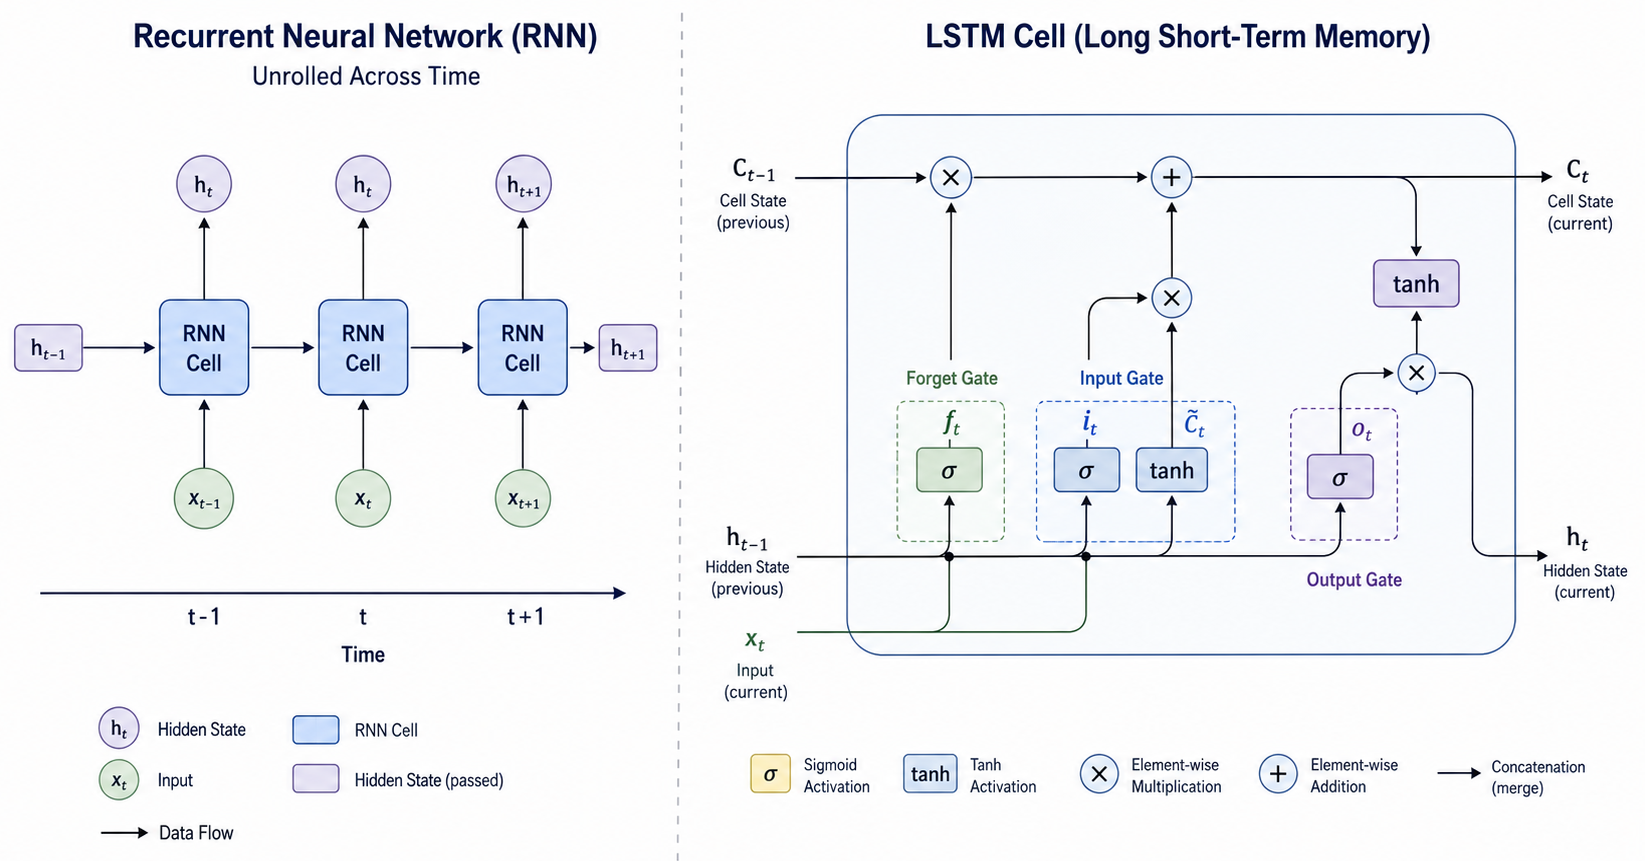
\includegraphics[width=1.0\textwidth]{ressources/chapter2/RNN_vs_LSTM.png}
    \caption{Architecture of RNN and LSTM.}
    \label{fig:rnn-lstm}
\end{figure}

\subsection{Transformer Architecture}

The transformer architecture, introduced by Vaswani et al.~\cite{vaswani2017attention}, has become the dominant model for sequence processing tasks. Unlike RNNs, which process sequences sequentially, the transformer processes all positions simultaneously using \textit{self-attention}. The core operation is \textit{scaled dot-product attention}:

\begin{equation}
    \text{Attention}(Q, K, V) = \text{softmax}\!\left(\frac{QK^T}{\sqrt{d_k}}\right) V
\end{equation}

where $Q$ (query), $K$ (key), and $V$ (value) are learned linear projections of the input. The dot product $QK^T$ measures the compatibility between each pair of positions; the softmax normalizes these into attention weights; and the weighted sum of values produces the output. The scaling factor $1/\sqrt{d_k}$ prevents the dot products from growing too large, which would push the softmax into regions of vanishing gradients.

\textbf{Multi-head attention} extends this by applying $h$ parallel attention operations with different learned projections, allowing the model to attend to information from different representation subspaces simultaneously:

\begin{equation}
    \text{MultiHead}(Q, K, V) = \text{Concat}(\text{head}_1, \ldots, \text{head}_h) W^O
\end{equation}

where $\text{head}_i = \text{Attention}(QW_i^Q, KW_i^K, VW_i^V)$.

A transformer layer consists of multi-head self-attention followed by a position-wise feedforward network, with residual connections and layer normalization around each sub-layer. Multiple such layers are stacked to form the full transformer encoder. In our system, the transformer encoder replaces the \gls{lstm} for encoding loop nest features, using structured tokenization where each loop level is treated as a token and positional encodings capture the depth and role of each token in the nest hierarchy.

\begin{figure}[H]
    \centering
    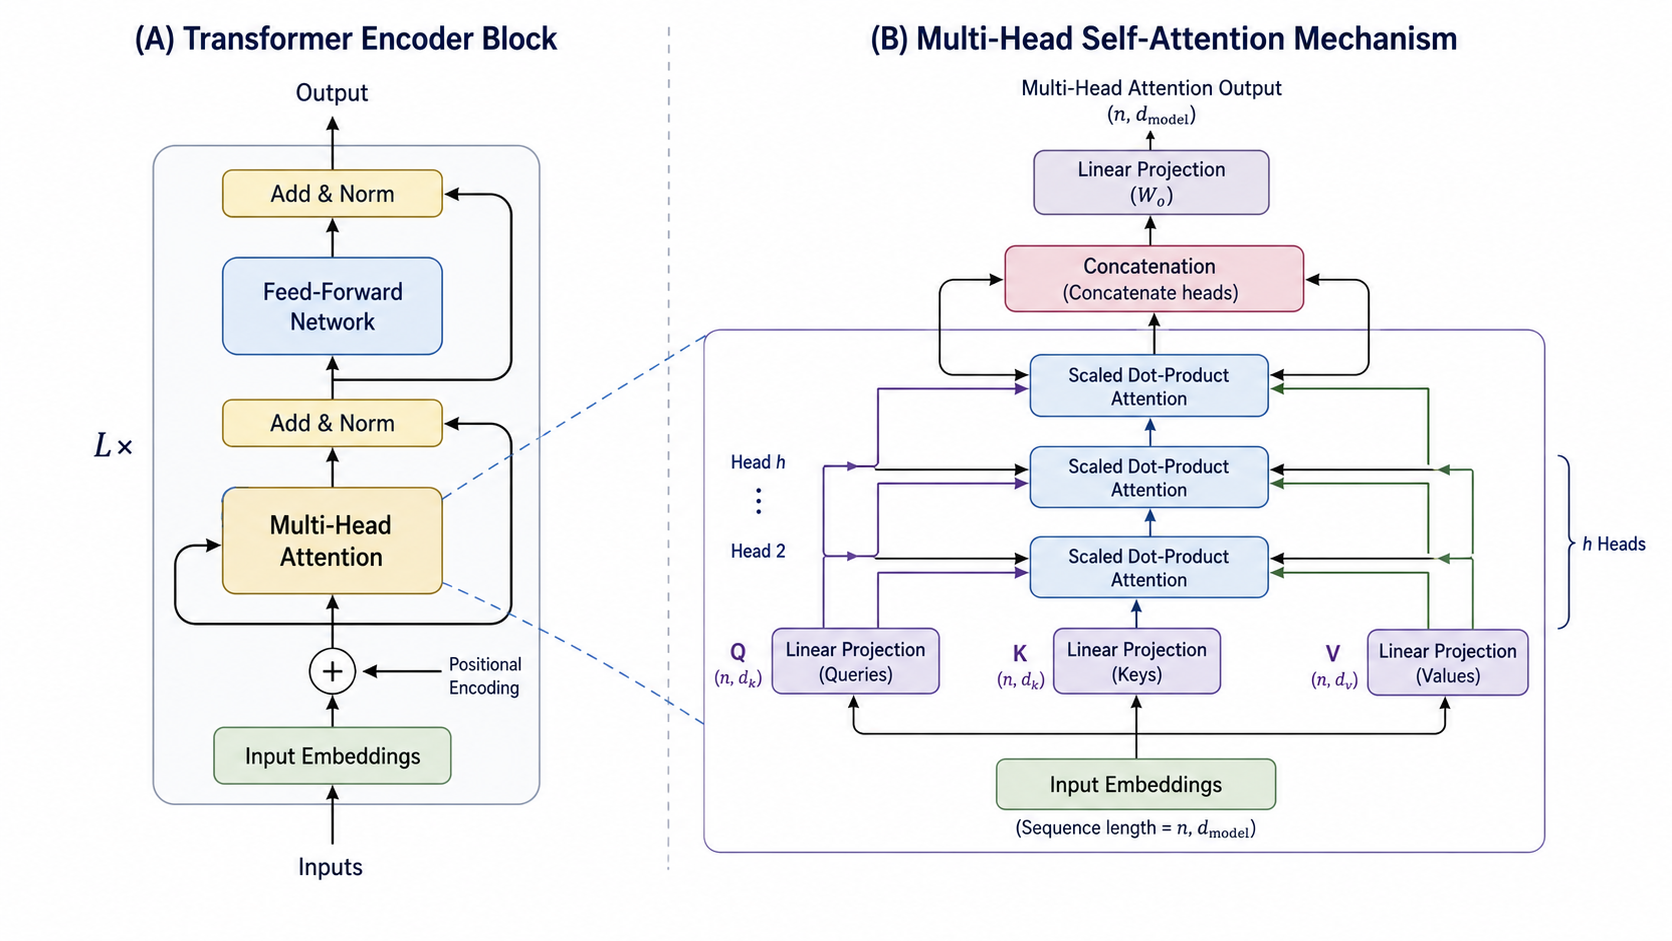
\includegraphics[width=1.0\textwidth]{ressources/chapter2/transformer_encoder_and_attention_mechanism.png}
    \caption{The Transformer architecture detailing the multi-head self-attention mechanism.}
    \label{fig:transformer-arch}
\end{figure}

\section{The Reinforcement Learning Framework}

Reinforcement learning formalizes the problem of learning through interaction to achieve a goal~\cite{sutton2018reinforcement}. This section introduces the core mathematical framework and concepts.

\subsection{Markov Decision Processes}

The standard formalism for \gls{rl} is the \gls{mdp}. An \gls{mdp} is defined by the tuple $(\mathcal{S}, \mathcal{A}, \mathcal{P}, \mathcal{R}, \gamma)$, where:

\begin{itemize}
    \item $\mathcal{S}$ is the set of \textit{states} that the environment can be in.
    \item $\mathcal{A}$ is the set of \textit{actions} available to the agent.
    \item $\mathcal{P}(s' \mid s, a)$ is the \textit{transition function}, giving the probability of transitioning to state $s'$ after taking action $a$ in state $s$.
    \item $\mathcal{R}(s, a, s')$ is the \textit{reward function}, giving the immediate reward received after transitioning from $s$ to $s'$ via action $a$.
    \item $\gamma \in [0, 1]$ is the \textit{discount factor}, which trades off the importance of immediate versus future rewards.
\end{itemize}

The Markov property states that the future depends only on the current state and action, not on the history of previous states. Formally, $\mathcal{P}(s_{t+1} \mid s_t, a_t) = \mathcal{P}(s_{t+1} \mid s_t, a_t, s_{t-1}, a_{t-1}, \ldots, s_0, a_0)$. In our compiler optimization setting, the state captures all relevant information about the current state of the \gls{mlir} code and the optimization history, satisfying this property.

\subsection{Agents and Environments}

At each discrete time step $t$, the agent and environment interact as follows:

\begin{enumerate}
    \item The agent observes the current state $s_t \in \mathcal{S}$ of the environment.
    \item Based on $s_t$, the agent selects an action $a_t \in \mathcal{A}(s_t)$, where $\mathcal{A}(s_t)$ is the set of actions available in state $s_t$ (the \textit{action mask}).
    \item The environment transitions to a new state $s_{t+1}$ and emits a reward $r_{t+1} \in \mathbb{R}$.
    \item The agent receives $s_{t+1}$ and $r_{t+1}$, and the cycle repeats.
\end{enumerate}

This interaction loop, illustrated in Figure~\ref{fig:rl-loop}, continues until the agent reaches a \textit{terminal state} (the episode ends) or a predefined horizon is reached.

\begin{figure}[H]
    \centering
    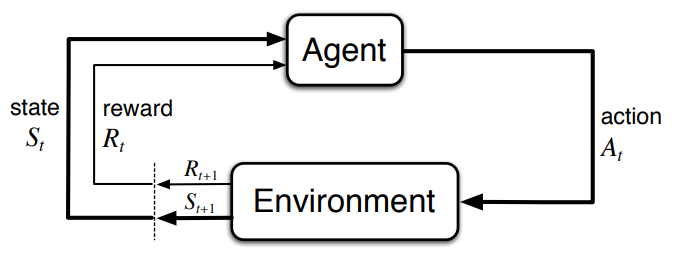
\includegraphics[width=0.7\textwidth]{ressources/chapter2/reinforcement_learning_feedback_loop.png}
    \caption{The reinforcement learning feedback loop. \cite{sutton2018reinforcement}}
    \label{fig:rl-loop}
\end{figure}

In our compiler optimization environment, the agent is the \gls{ppo} policy network, the environment is the \gls{mlir} compiler and execution engine, the state is the structured observation of the current Linalg operation and its context, the actions are loop transformations with their parameters, and the reward is a function of the achieved execution time speedup.

\subsection{Policy and Value Functions}

A \textit{policy}, denoted $\pi$, is the agent's strategy: given the current state $s$, it decides which action $a$ to take. Formally, a policy maps each state to a probability distribution over actions:

\begin{equation}
    \pi(a \mid s) = P(A_t = a \mid S_t = s)
\end{equation}

In plain terms, $\pi(a \mid s)$ answers the question: "If I am in state $s$, how likely am I to choose action $a$?" A policy can be \textit{deterministic} (always selecting the same action in a given state) or \textit{stochastic} (selecting actions according to a probability distribution). Stochastic policies are essential for exploration: by occasionally trying suboptimal actions, the agent discovers strategies it would otherwise miss.

The agent's goal is to find an \textit{optimal policy} $\pi^*$ that maximizes the cumulative reward collected over time. The total reward from time step $t$ onward, called the \textit{return} $G_t$, is:

\begin{equation}
    G_t = r_{t+1} + \gamma r_{t+2} + \gamma^2 r_{t+3} + \cdots = \sum_{k=0}^{\infty} \gamma^k r_{t+k+1}
\end{equation}

Here, $r_{t+1}$ is the immediate reward after the first action, $r_{t+2}$ is the reward one step later, and so on. The \textit{discount factor} $\gamma \in [0, 1]$ controls how much future rewards matter: $\gamma = 1$ means all rewards are equally important, while $\gamma = 0$ makes the agent care only about the immediate reward. Multiplying by $\gamma^k$ ensures that rewards $k$ steps in the future contribute less than near-term rewards, which reflects the intuition that a reward now is worth more than the same reward later.

To evaluate how good a given state is, we define the \textit{state-value function} $V^\pi(s)$, which estimates the expected return when starting in state $s$ and following policy $\pi$ thereafter:

\begin{equation}
    V^\pi(s) = \mathbb{E}_\pi\left[ G_t \mid S_t = s \right]
\end{equation}

The notation $\mathbb{E}_\pi[\cdot]$ denotes an \textit{expectation} under policy $\pi$: since both the environment transitions and the policy's action choices are probabilistic, $V^\pi(s)$ averages over all possible futures starting from $s$.

A related concept is the \textit{action-value function} $Q^\pi(s, a)$, which estimates the expected return when taking a specific action $a$ in state $s$ and then following policy $\pi$ afterwards:

\begin{equation}
    Q^\pi(s, a) = \mathbb{E}_\pi\left[ G_t \mid S_t = s, A_t = a \right]
\end{equation}

While $V^\pi(s)$ evaluates the state itself, $Q^\pi(s, a)$ evaluates a specific action choice, it answers: "If I take action $a$ now and follow the policy from then on, what total reward should I expect?"

The value functions obey a recursive relationship known as the \textit{Bellman equation}. Intuitively, the value of a state equals the immediate reward expected from the next action, plus the discounted value of the resulting next state:

\begin{equation}
    V^\pi(s) = \sum_a \pi(a \mid s) \sum_{s'} \mathcal{P}(s' \mid s, a) \left[ \mathcal{R}(s, a, s') + \gamma V^\pi(s') \right]
\end{equation}

Reading from left to right: for each possible action $a$ (weighted by how often the policy selects it, $\pi(a \mid s)$), consider each possible next state $s'$ (weighted by the environment's transition probability $\mathcal{P}(s' \mid s, a)$). The value is the immediate reward $\mathcal{R}(s, a, s')$ plus the discounted value of the next state $\gamma V^\pi(s')$. This recursive structure is what enables learning: the value of any state can be expressed in terms of the values of its successors.

The \textit{optimal} value functions $V^*$ and $Q^*$ are those achieved by the best possible policy $\pi^*$. They satisfy the Bellman optimality equation, which replaces the policy's action weighting with a maximization over actions:

\begin{equation}
    Q^*(s, a) = \sum_{s'} \mathcal{P}(s' \mid s, a) \left[ \mathcal{R}(s, a, s') + \gamma \max_{a'} Q^*(s', a') \right]
\end{equation}

This equation says: the value of taking action $a$ in state $s$ is the immediate reward plus the discounted value of the best possible action in the next state. The $\max_{a'}$ operator reflects optimal behavior---in state $s'$, the optimal agent will always pick the action with the highest Q-value.

\subsection{Exploration vs.\ Exploitation}

A fundamental tension in reinforcement learning is the \textit{exploration-exploitation trade-off}. To maximize cumulative reward, the agent should \textit{exploit} its current knowledge by selecting actions that it believes are best. However, to discover better actions, the agent must also \textit{explore} by trying actions whose outcomes are uncertain.

Common exploration strategies include:

\begin{itemize}
    \item \textbf{$\epsilon$-greedy}: With probability $\epsilon$, select a random action; otherwise, select the action with the highest estimated value. The parameter $\epsilon$ is typically decayed over time as the agent's knowledge improves.
    \item \textbf{Entropy regularization}: Add a bonus to the policy optimization objective proportional to the entropy of the policy distribution, encouraging the policy to remain stochastic and continue exploring. This is the primary exploration mechanism in \gls{ppo} and in our system.
\end{itemize}

Our \gls{ppo} agent uses a combination of entropy regularization and optional $\epsilon$-greedy exploration, with $\epsilon$ decaying linearly from an initial value to a small final value over the course of training.

\section{Types of Reinforcement Learning Algorithms}

\gls{rl} algorithms can be classified along several axes. Understanding these categories helps contextualize the choice of \gls{ppo} for our system.

\subsection{Model-Based vs.\ Model-Free RL}

\textbf{Model-based} methods learn or use an explicit model of the environment's dynamics—the transition function $\mathcal{P}$ and reward function $\mathcal{R}$. With a model, the agent can plan ahead by simulating possible futures before acting. Model-based methods are typically more sample-efficient but require learning an accurate model, which is challenging in complex environments.

\textbf{Model-free} methods learn a policy or value function directly from experience without explicitly modeling the environment's dynamics. They are simpler to implement and have been more successful in high-dimensional domains, but they typically require more environment interactions to learn. \gls{ppo} is a model-free algorithm: the agent learns directly from the rewards obtained by executing transformation sequences, without attempting to model the compiler's behavior.

\subsection{Value-Based vs.\ Policy-Based Methods}

\textbf{Value-based} methods learn the optimal action-value function $Q^*$ and derive a policy implicitly by selecting actions that maximize $Q^*$ (e.g., $\pi(s) = \arg\max_a Q(s, a)$). Q-Learning and \gls{dqn} are value-based methods. They are effective for discrete action spaces but can struggle with continuous actions and stochastic policies.

\textbf{Policy-based} methods learn an explicit parameterized policy $\pi_\theta(a \mid s)$ directly, optimizing the policy parameters $\theta$ to maximize expected return. Pure policy gradient methods (e.g., REINFORCE) fall into this category. They naturally handle stochastic policies and can be extended to continuous action spaces, making them well-suited for hierarchical action spaces.

\textbf{Actor-critic} methods combine value-based and policy-based approaches. An \textit{actor} (the policy) selects actions, while a \textit{critic} (the value function) evaluates the quality of those actions. The critic's evaluation provides a lower-variance learning signal for the actor compared to pure policy gradient methods. \gls{ppo} is an actor-critic algorithm.

\subsection{On-Policy vs.\ Off-Policy Methods}

\textbf{On-policy} methods learn about the policy currently being followed by the agent. Data used for training must be collected under the current policy, and old data becomes stale when the policy changes. On-policy methods are typically more stable but less sample-efficient because they cannot reuse past experience.

\textbf{Off-policy} methods can learn from data collected under a different (behavior) policy. This enables experience replay, where transitions are stored in a buffer and sampled repeatedly for training, significantly improving sample efficiency. Q-Learning and \gls{dqn} are off-policy methods; REINFORCE is on-policy.

\gls{ppo} occupies an intermediate position: it is fundamentally on-policy (trajectories are collected under the current policy and used for a limited number of gradient updates), but its clipped objective allows for moderate policy changes without requiring fresh data, and our implementation includes optional experience replay to improve sample efficiency.

\section{Key Reinforcement Learning Algorithms}

This section presents the specific algorithms that form the foundation of modern deep \gls{rl} and are most relevant to our work.

\subsection{Q-Learning}

Q-Learning, introduced by Watkins and Dayan~\cite{watkins1992qlearning}, is a model-free, off-policy, value-based algorithm. It learns the optimal action-value function $Q^*$ through \gls{td} learning. The update rule is:

\begin{equation}
    Q(s_t, a_t) \leftarrow Q(s_t, a_t) + \alpha \left[ r_{t+1} + \gamma \max_{a'} Q(s_{t+1}, a') - Q(s_t, a_t) \right]
\end{equation}

where $\alpha$ is the learning rate. The term in brackets is the \textit{\gls{td} error}: the difference between the current estimate $Q(s_t, a_t)$ and the target $r_{t+1} + \gamma \max_{a'} Q(s_{t+1}, a')$, which uses the maximum Q-value of the next state (the off-policy component, since the target assumes optimal future behavior regardless of the agent's actual policy).

Q-Learning is guaranteed to converge to $Q^*$ in the tabular case (finite state and action spaces) under standard stochastic approximation conditions~\cite{watkins1992qlearning}. However, tabular methods are limited to problems with small, discrete state spaces—a condition that compiler optimization, with its high-dimensional state representation, does not satisfy.

\subsection{Deep Q-Networks}

Deep Q-Networks, introduced by Mnih et al.~\cite{mnih2015human}, extend Q-Learning to high-dimensional state spaces by approximating the Q-function with a deep neural network: $Q(s, a; \theta) \approx Q^*(s, a)$. \gls{dqn} introduced two key innovations to stabilize training with non-linear function approximators:

\begin{enumerate}
    \item \textbf{Experience replay}: Transitions $(s_t, a_t, r_{t+1}, s_{t+1})$ are stored in a replay buffer and sampled uniformly at random for training. This breaks the correlation between consecutive samples and allows each transition to be used for multiple updates, improving sample efficiency.

    \item \textbf{Target network}: A separate \textit{target network} $Q(s, a; \theta^-)$ with parameters $\theta^-$ is used to compute the \gls{td} target. The target network's parameters are periodically copied from the online network ($\theta^- \leftarrow \theta$) and held fixed between updates, preventing the target from changing during optimization and reducing instability.
\end{enumerate}

The \gls{dqn} loss function is:

\begin{equation}
    \mathcal{L}(\theta) = \mathbb{E}_{(s, a, r, s') \sim \mathcal{D}}\left[ \left( r + \gamma \max_{a'} Q(s', a'; \theta^-) - Q(s, a; \theta) \right)^2 \right]
\end{equation}

where $\mathcal{D}$ is the replay buffer. \gls{dqn} demonstrated human-level performance on a suite of Atari games and established deep \gls{rl} as a viable approach for complex sequential decision-making problems. However, \gls{dqn} is limited to discrete action spaces and does not directly learn a stochastic policy, which is desirable in our setting for exploration and for handling the hierarchical action structure.

\subsection{Policy Gradient Methods}

Policy gradient methods directly optimize the policy parameters $\theta$ to maximize expected return. The fundamental result is the \textit{policy gradient theorem}~\cite{sutton1999policy}:

\begin{equation}
    \nabla_\theta J(\theta) = \mathbb{E}_\pi \left[ \nabla_\theta \log \pi_\theta(a \mid s) \, \Psi_t \right]
\end{equation}

where $\Psi_t$ is a quantity that evaluates the quality of action $a$ in state $s$. Different choices of $\Psi_t$ yield different algorithms:

\begin{itemize}
    \item \textbf{REINFORCE}~\cite{williams1992simple}: Uses the Monte Carlo return $G_t$ as $\Psi_t$. Unbiased but high variance.
    \item \textbf{Actor-critic}: Uses the advantage $A_t = Q(s_t, a_t) - V(s_t)$ as $\Psi_t$. The advantage measures how much better action $a_t$ is compared to the average action in state $s_t$, reducing variance by subtracting the state baseline $V(s_t)$.
\end{itemize}

\textbf{REINFORCE} is the simplest policy gradient algorithm. After collecting a full episode, it updates the policy parameters:

\begin{equation}
    \theta \leftarrow \theta + \eta \sum_{t=0}^{T} \nabla_\theta \log \pi_\theta(a_t \mid s_t) \, G_t
\end{equation}

While simple and unbiased, REINFORCE suffers from high variance in the gradient estimates, leading to slow and unstable learning. Actor-critic methods reduce this variance, and \gls{ppo} further improves stability through a clipped objective.

\subsection{Generalized Advantage Estimation}

Generalized Advantage Estimation~\cite{schulman2015gae} computes advantage estimates that dynamically balance bias and variance. The \gls{gae} advantage at time $t$ uses the one-step \gls{td} error $\delta_t = r_{t+1} + \gamma V(s_{t+1}) - V(s_t)$, discounted exponentially using the hyperparameter $\lambda \in [0, 1]$:

\begin{equation}
    \hat{A}_t^{\text{GAE}(\gamma, \lambda)} = \sum_{l=0}^{\infty} (\gamma \lambda)^l \delta_{t+l} = \delta_t + \gamma \lambda \hat{A}_{t+1}
\end{equation}

By tuning $\lambda$, \gls{gae} transitions smoothly between the low-variance but potentially biased 1-step \gls{td} error ($\lambda = 0$) and the unbiased, high-variance Monte Carlo return ($\lambda = 1$). Our agent utilizes \gls{gae} to provide robust baseline subtraction during policy updates.

\subsection{Proximal Policy Optimization}

Proximal Policy Optimization, introduced by Schulman et al.~\cite{schulman2017ppo}, is the \gls{rl} algorithm used in our system. \gls{ppo} addresses a central challenge in policy gradient methods: how to take the largest possible improvement step on the policy without causing a collapse in performance due to excessively large updates. It limits the magnitude of policy updates using a clipped surrogate objective while relying on an actor-critic structure.

To formalize this, algorithm~\ref{alg:ppo} details the exact procedure by which \gls{ppo} alternates between trajectory collection and multiple epochs of stochastic gradient ascent on the clipped loss.

\begin{algorithm}[H]
\caption{Proximal Policy Optimization}\label{alg:ppo}
\textbf{Input:} clipping threshold $\epsilon$, policy learning rate $\alpha$, value learning rate $\beta$, entropy coefficient $c_2$, value loss coefficient $c_1$. \\
\textbf{Output:} Optimized policy $\pi_\theta(a \mid s)$
\begin{algorithmic}
\State Initialize policy $\pi_\theta$ and value function $V_\phi$
\For{each iteration}
    \State Collect trajectory $\{s_t, a_t, r_t\}_{t=0}^T$ using current policy $\pi_\theta$
    \State Compute the advantage estimates $\hat{A}_t$ using \gls{gae} (and targets $V_t^{\text{target}}$)
    \For{each epoch}
        \For{each minibatch}
            \State Compute ratio: $r_t(\theta) = \frac{\pi_\theta(a_t \mid s_t)}{\pi_{\theta_{\text{old}}}(a_t \mid s_t)}$
            \State Clipped surrogate objective: $\mathcal{L}^{\text{CLIP}}(\theta) = \hat{\mathbb{E}} \left[ \min\left( r_t(\theta) \hat{A}_t, \, \text{clip}(r_t(\theta), 1 - \epsilon, 1 + \epsilon)\hat{A}_t \right) \right]$
            \State Value function loss: $\mathcal{L}^{\text{VF}}(\phi) = \hat{\mathbb{E}} \left[ \left(V_\phi(s_t) - V_t^{\text{target}}\right)^2 \right]$
            \State Entropy loss: $\mathcal{L}^{\text{Entropy}}(\theta) = - \sum_a \pi_\theta(a \mid s_t)\log(\pi_\theta(a \mid s_t))$
            \State Total loss: $\mathcal{L} = \mathcal{L}^{\text{CLIP}}(\theta) - c_1 \mathcal{L}^{\text{VF}}(\phi) + c_2 \mathcal{L}^{\text{Entropy}}(\theta)$
            \State Update $\theta, \phi$ using stochastic gradient optimization on $\mathcal{L}$
        \EndFor
    \EndFor
\EndFor
\end{algorithmic}
\end{algorithm}


The clipping mechanism in the objective $\mathcal{L}^{\text{CLIP}}(\theta)$ bounds how much the probability ratio $r_t(\theta)$ can vary:
\begin{itemize}
    \item If the advantage $\hat{A}_t$ is positive (the action was better than expected), the objective is clipped at $1 + \epsilon$, preventing the policy from increasing the probability of that action too aggressively.
    \item If the advantage $\hat{A}_t$ is negative (the action was worse than expected), the objective is clipped at $1 - \epsilon$, preventing the policy from decreasing the probability too aggressively.
    \item The $\min$ operation ensures that the final objective is a lower (pessimistic) bound on the unclipped objective, making the update conservative.
\end{itemize}

The full \gls{ppo} loss function used in our implementation includes additional terms:

\begin{equation}
    \mathcal{L}(\theta) = \mathcal{L}^{\text{CLIP}}(\theta) - c_1 \mathcal{L}^{\text{VF}}(\theta) + c_2 \mathcal{H}[\pi_\theta](\cdot \mid s_t)
\end{equation}

where:

\begin{itemize}
    \item $\mathcal{L}^{\text{VF}}(\theta) = (V_\theta(s_t) - V_t^{\text{target}})^2$ is the value function loss (mean squared error between predicted and target values). Our system optionally applies value clipping: $\text{clip}(V_\theta(s_t), V_{\text{old}}(s_t) - \epsilon_v, V_{\text{old}}(s_t) + \epsilon_v)$ to prevent large value updates.
    \item $\mathcal{H}[\pi_\theta](\cdot \mid s_t) = -\sum_a \pi_\theta(a \mid s_t) \log \pi_\theta(a \mid s_t)$ is the entropy of the policy, used as an exploration bonus. The coefficient $c_2$ controls the strength of entropy regularization.
    \item $c_1$ is the value function coefficient balancing the policy and value losses.
\end{itemize}

\textbf{Training procedure.} \gls{ppo} training proceeds in iterations, each consisting of:

\begin{enumerate}
    \item \textbf{Trajectory collection}: The current policy $\pi_{\theta_{\text{old}}}$ is used to interact with the environment for a fixed number of time steps, collecting trajectories of $(s_t, a_t, r_{t+1})$.
    \item \textbf{Advantage computation}: Advantages $\hat{A}_t$ are computed using \gls{gae}, and value targets are computed from the returns.
    \item \textbf{Policy update}: The policy and value networks are updated for $K$ epochs (typically $K = 4$ in our system) using mini-batches sampled from the collected trajectories, optimizing the \gls{ppo} objective with Adam.
    \item \textbf{Repeat}: A new iteration begins with the updated policy.
\end{enumerate}

\gls{ppo} has become one of the most widely used \gls{rl} algorithms due to its simplicity, stability, and strong empirical performance across a range of domains~\cite{berner2019dota}. These properties make it well-suited for compiler optimization, where training is computationally expensive and stability is important: the clipped objective reduces the risk of destabilizing policy collapse during training, and the on-policy nature ensures that the agent is always evaluated on data representative of its current behavior.

\begin{table}[H]
    \centering
    \caption{Summary of reinforcement learning algorithms discussed in this chapter.}
    \label{tab:rl-algorithms}
    \vspace{0.2cm}
    \begin{tabularx}{\textwidth}{l l l l >{\raggedright\arraybackslash}p{4cm}}
        \toprule
        \textbf{Algorithm} & \textbf{Type} & \textbf{Policy} & \textbf{Action Space} & \textbf{Key Features} \\
        \midrule
        Q-Learning & Value-based & Off-policy & Discrete & Tabular, guaranteed convergence \\
        \addlinespace
        \gls{dqn} & Value-based & Off-policy & Discrete & Experience replay, target network \\
        \addlinespace
        REINFORCE & Policy-based & On-policy & Discrete / Continuous & Simple, unbiased, high variance \\
        \addlinespace
        \gls{ppo} & Actor-critic & On-policy & Discrete / Continuous & Clipped objective, entropy bonus, stable \\
        \bottomrule
    \end{tabularx}
\end{table}

\section{Conclusion}

This chapter introduced \gls{rl} as the algorithmic foundation of our compiler optimization framework. We defined the interaction loop consisting states, actions, rewards, and transitions, formalized as a Markov Decision Process. 

By detailing value and policy functions, alongside advancements like generalized advantage estimation, we established the need for robust learning policies. We highlighted \gls{ppo}; our actor-critic algorithm of choice, which uses clipped objectives to stabilize learning and effectively balance exploration versus exploitation through entropy regularization. These properties make \gls{ppo} exceptionally well-suited for the noisy, high-dimensional search spaces inherent in compiler optimization.

With the necessary \gls{rl} concepts formalized, the subsequent chapter surveys the state-of-the-art literature, situating our \gls{ppo}-based agent against existing machine-learning-driven compiler optimizations and defining our distinct contributions.
